\documentclass{article}

\usepackage{tikz}
\usepackage{amsfonts}
\usepackage{amssymb}

\usepackage[english]{babel}
\usepackage[autostyle]{csquotes}
\MakeOuterQuote{"}

\title{The Calculus of Constructions, EliDupree Edition}
\author{Eli Dupree}
\date{\today}

\newcommand{\Prop}{\mathbb{P}}
\newcommand{\istype}{\ \mathrm{type}}
\newcommand{\usage}{\mathcal{V}}
\newcommand{\usageKnown}[2]{(\usage[#2:#1])}
\newcommand{\presep}{\hspace{1.8em}}
\newcommand{\subst}[3]{#1[#2:=#3]}
\newcommand{\subty}[1]{#1^*}
\newcommand{\bindvariable}{\bigstar}
\newcommand{\bindnotthis}{\circ}

\begin{document}
  \maketitle

  \section{Fundamentals}
  \subsection{Formulas}

  The Calculus of Constructions (CoC) is a system of formulas. The following context-free grammar shows the six elementary "formula constructors" – ways to build a formula, sometimes from smaller formulas ($F$):

  \[ F \rightarrow \Prop \mid \usage \mid \usageKnown{F}{i} \mid \lambda b:F,F \mid \forall b:F,F \mid (F F) \]
  
  By combining these constructors into larger formulas, you can express all of computation and mathematics. Our definitions are mainly concerned with judging which of these formulas are \textbf{types}, and which other formulas are \textbf{members} of those types. Anywhere you see the symbol $:$, as in $v : T$, it means a claim that something is a member of the type $T$.

  Here is an informal description of each formula constructor:

  $\Prop$ (read as "Prop") is the \emph{type of all ordinary types}. It's called "Prop" because the ordinary types can represent \emph{propositions} (although they can represent many other things as well).
  
  $\lambda b:T,v$ ("a lambda") is a \emph{function} which maps a single parameter, of type $T$, to the formula $v$ (after the value of the parameter is substituted into $v$) We call $T$ the \textbf{parameter type}, and $v$ the \textbf{body} or \textbf{return value}.
  
  $\forall b:T,U$ ("a forall", read as "for all $b$ in $T$, $U$") is the \emph{type} of any $\lambda c:T,v$ where $v : U$. It's called a forall because of the way that types can represent propositions: The members of a type are the proofs of a proposition, and a proposition with no proofs (an empty type) is a false proposition\footnote{A fan of Gödel might ask: "What about propositions that are true but unprovable?" Well, we are free to define "true" to mean "provable within CoC"; we are speaking of \emph{constructive} truth, which is a slightly stronger claim than truth in classical logic. Like all theories, CoC must be incomplete, but the form of that incompleteness is just that there are some propositions $P$ where neither $P$ nor $\neg P$ is provable.}. If the proposition $U$ is true for all members of the type $T$, then you can write a lambda that maps any member of $T$ to a member of $U$, and that lambda will be a member (a proof) of $\forall b:T,U$. As with lambdas, we call $T$ the \textbf{parameter type}, and $U$ the \textbf{body} or \textbf{return type}.
  
  $\usage$ is a \emph{variable usage}, which may appear inside the body of a lambda or forall, as a location to substitute in the value of the parameter. $\usageKnown{T}{i}$ is the same, but with an explicit definition of its type and variable-identity.
  
  $(f v)$ is a \emph{function application} – the kind that would be written $f(v)$ in the notation of usual math or programming. CoC descends from the lambda calculus, where this is written as $f v$.
  
  Before we can make these definitions formal, we must take a couple of detours.  

  \subsection{Variable identities}

  You may note that I haven't defined $b$ (or $i$). If you know lambda calculus, you're expecting $b$ to be a variable name. Due to some definitional inconveniences\footnote{Using variable names requires you to define "alpha-conversions" and "contexts", and to make substitutions allow renaming bindings. Our formulation allows us to dispense with these complications – at the price of a somewhat-smaller amount of complications.}, we use a different (yet equivalent) definition. $b$ is a \textbf{binding tree}, with the following grammar:

  \[b \rightarrow \bindvariable \mid \bindnotthis \mid (b b) \]

  This requires some explanation. In the usual lambda calculus, you may write

  \[ \lambda x : \mathrm{Number}, ((\mathrm{plus}\ 2)\ x) \]

  to mean the function which maps any number to the same number plus 2. This expression uses the symbol $x$ in two different ways: the first occurrence of $x$ is a \textbf{binding}, introducing a new variable that will henceforth be called "$x$". The second occurrence of $x$ is a \textbf{usage}, saying to substitute in the value that was previously named "$x$". Similarly, if you want a function with multiple parameters, you may write
  
  \[ \lambda x : \mathrm{Number}, \lambda y : \mathrm{Number}, ((\mathrm{plus}\ x)\ y) \]

  In our definitions, all \textbf{usages} are the exact same formula $\usage$, so this becomes
  
  \[ \lambda x, \lambda y, ((\mathrm{plus}\ \usage)\ \usage) \]
  
  So how do you tell that it's $x + y$, rather than $x + x$ or $y + y$? The answer is that our \textbf{bindings}, $x$ and $y$ themselves, tell you this. The full expansion is this:
  
  \[ \lambda (\bindnotthis((\bindnotthis \bindvariable) \bindnotthis)) : \mathrm{Number}, \lambda ((\bindnotthis \bindnotthis) \bindvariable) : \mathrm{Number}, ((\mathrm{plus}\ \usage)\ \usage) \]
  
  This is best visualized as a tree, where each lambda's binding-tree is the \emph{same shape} as the whole body of that lambda:
  
  [TODO: construct the diagram when I'm in a better position to do that relative to my computer]
  
  Observe that it is straightforward to convert between the "variable names" form and the "binding trees" form:
  \begin{itemize}
    \item If you are given variable names, you can write binding trees that place $\bindvariable$ at the locations of the usages with the same name.
    \item If you are given binding trees, you can give each binding a name, and write that name on each usage where there was a $\bindvariable$.
  \end{itemize}
  
  
  \subsection{Type judgments}
    
  
  \[ \frac{\emptyset}{\Prop\istype} \]
  \[ \frac{T : \Prop}{T\istype} \]
  \[ \frac{T\istype}{\usageKnown{T}{i}:T} \]
  \[ \frac{T\istype\presep \subty{U}\istype}{(\forall b:T,U)\istype} \]
  \[ \frac{T\istype\presep \subty{U} : \Prop}{(\forall b:T,U) : \Prop} \]
  \[ \frac{\subty{v} : \subty{U} \presep (\forall b:T,U)\istype}{(\lambda c:T,v) : (\forall b:T,U)} \]
  \[ \frac{f : (\forall b:T,U) \presep v : T}{(f v) : \subst{U}{b}{v}} \]
  

  \section{Type relationships}
  All complete\footnote{A "complete" formula is one where the types of all free variables are known.} formulas of CoC can be immediately\footnote{By a process that is $O(n)$ in the size of the formula.} classified into one of the following groups.

  \vspace{0.5cm}

  \noindent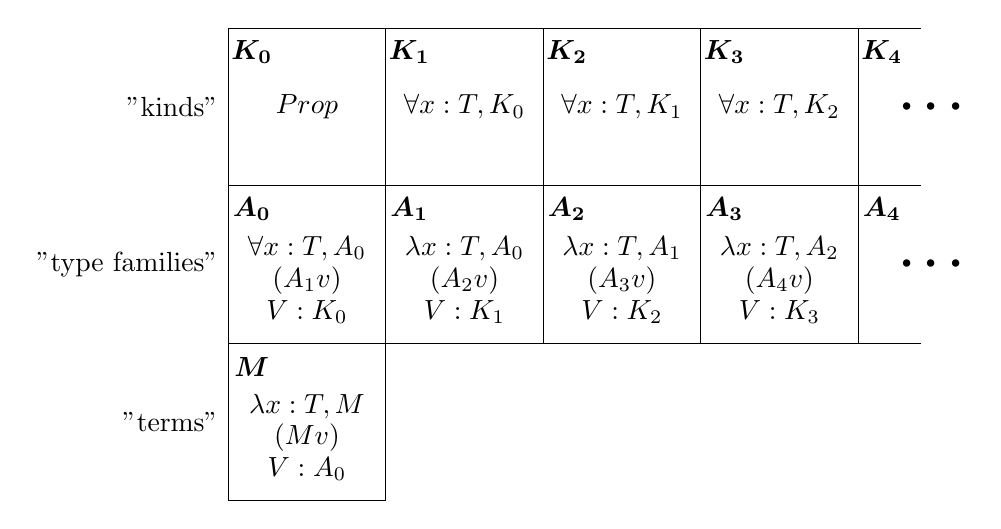
\begin{tikzpicture}
    \pgfsetxvec{\pgfpoint{2cm}{0}}
    \pgfsetyvec{\pgfpoint{0}{-2cm}}

    \draw (0,0.5) node[left]{"kinds"};
    \draw (0,1.5) node[left]{"type families"};
    \draw (0,2.5) node[left]{"terms"};
    \foreach \y in {0,1,2} {
      \draw (0,\y) rectangle (1,\y+1);
      \draw (4,\y) -- (4.4,\y);
    }
    \foreach \y in {0,1} {
      \draw (4.2,\y+0.5) node[right]{{\LARGE \boldmath $\cdots$}};
    }
    \foreach \x in {0,1,2,3,4} {
      \draw (\x+0.15,0.15) node[]{{\boldmath $K_\x$}};
      \draw (\x+0.15,1.15) node[]{{\boldmath $A_\x$}};
    }
    \foreach \x in {0,1,2,3} {
      \draw (\x+0.5,1.8) node[]{$V : K_\x$};
    }
    \draw (0.15,2.15) node[]{{\boldmath $M$}};
    \draw (0.5,0.5) node[]{$Prop$};
    \draw (0.5,1.4) node[]{$\forall x:T,A_0$};
    \draw (0.5,1.6) node[]{$(A_1 v)$};
    \draw (0.5,2.4) node[]{$\lambda x:T,M$};
    \draw (0.5,2.6) node[]{$(M v)$};
    \draw (0.5,2.8) node[]{$V : A_0$};
    \foreach \l/\x/\r in {0/1/2,1/2/3,2/3/4} {
%      \pgfmathsetmacro{\l}{\x-1};
      \draw (\x,0) rectangle (\x+1,1);
      \draw (\x+0.5,0.5) node[]{$\forall x:T,K_{\l}$};
      \draw (\x,1) rectangle (\x+1,2);
      \draw (\x+0.5,1.4) node[]{$\lambda x:T,A_{\l}$};
      \draw (\x+0.5,1.6) node[]{$(A_{\r} v)$};
    }
  \end{tikzpicture}

  \vspace{0.5cm}

  In the above chart, $V:T$ denotes a variable-usage-site whose bound type is in the cell $T$. The literal $T$ can denote any \emph{type}, and $v$ can denote any \emph{value}, which we shall define forthwith. The other letters refer to cells; for example, $A_2$ can denote any formula from the cell $A_2$.

  If\footnote{In general, it may be very difficult to determine whether a formula has a type \emph{at all}. But it is easy (again, $O(n)$) to give any formula $V$ a \emph{provisional} type $T$, where if $V$ has any types at all, its types are exactly all the well-typed beta-conversions of $T$. The only difficult part is determining whether function arguments have the correct types.} a formula has a type, that type is in the cell directly above its own. Thus, the \emph{values} (formulas that can be members of types) include everything except the top row, and the \emph{types} (formulas that can have members) include everything except the bottom-most cells. As such, $A_0$ (the cell of propositions) is the unique cell whose formulas are both types and values.
\end{document}
